\documentclass[graphics]{beamer}

\usepackage{graphicx}
\usepackage{verbatim}
\usepackage{wrapfig}
\useoutertheme{shadow}
%\usecolortheme{orchid}
\usecolortheme{seahorse}


% math commands
\newcommand{\be}{\begin{eqnarray}}
\newcommand{\ee}{\end{eqnarray}}
\newcommand{\beq}{\begin{equation}}
\newcommand{\eeq}{\end{equation}}
\def\simless{\mathbin{\lower 3pt\hbox
      {$\rlap{\raise 5pt\hbox{$\char'074$}}\mathchar"7218$}}}
\def\simgreat{\mathbin{\lower 3pt\hbox
      {$\rlap{\raise 5pt\hbox{$\char'076$}}\mathchar"7218$}}} %> or of order

% variables

\def\toonscale{0.45}
\def\mboxy#1{\mbox{\small #1}}


\begin{comment}
\AtBeginSection[]{
  \frame{
    \frametitle{Outline}
    \tableofcontents[currentsection]
  }
}
\end{comment}

\title{Wave Optics, Imaginary Paths, Quantization
}
%\subtitle{interim update}
\author[U. Pen]{Ue-Li Pen
}
\date{December 14, 2021}


\begin{document}

%\section*{Introduction}
\section{Lenses}

\begin{comment}
  \subsection{Outline}

  \frame{
    \frametitle{Outline}
    \tableofcontents
  }
\end{comment}

\frame{\maketitle}



  \frame{
    \frametitle{Waves, Particles, Geodesics}
    \begin{itemize}
        \item Everything is a wave
        \item Short wavelength limit has classical particle
          interpretation: Eikonal
        \item Picard-Lefschetz: no waves, everything is a particle!
        \item New tool for FRBs, pulsars
        \item New picture for quantization: quantum gravity?
    \end{itemize}
  }


  \frame{
\vspace{-0.5in}
    \frametitle{History}
    \begin{itemize}
    \item Huygens, Fermat, Feynmann
    \item Picard-Lefschetz (19th century), Witten (2010)          
    \item concept: Oscillatory (Kirchoff) path integral
    \item sum over all possible paths, weighted by phase
    \item new phenomena: imaginary images, diffraction
    \item Eikonal: Dual description of waves by particles
    \end{itemize}
  }


  \frame{
\vspace{-0.25in}
    \frametitle{Optics: Geometric, Eikonal, Wave, P-L}
    \begin{itemize}
        \item Consider 1-D lens
        \item lensing potential $\Psi(\theta)$
        \item deflection $\Psi'$
        \item simplify for $D_{\rm ds}=\infty$
    \end{itemize}
\vspace{-0.5in}\hspace{2.5in}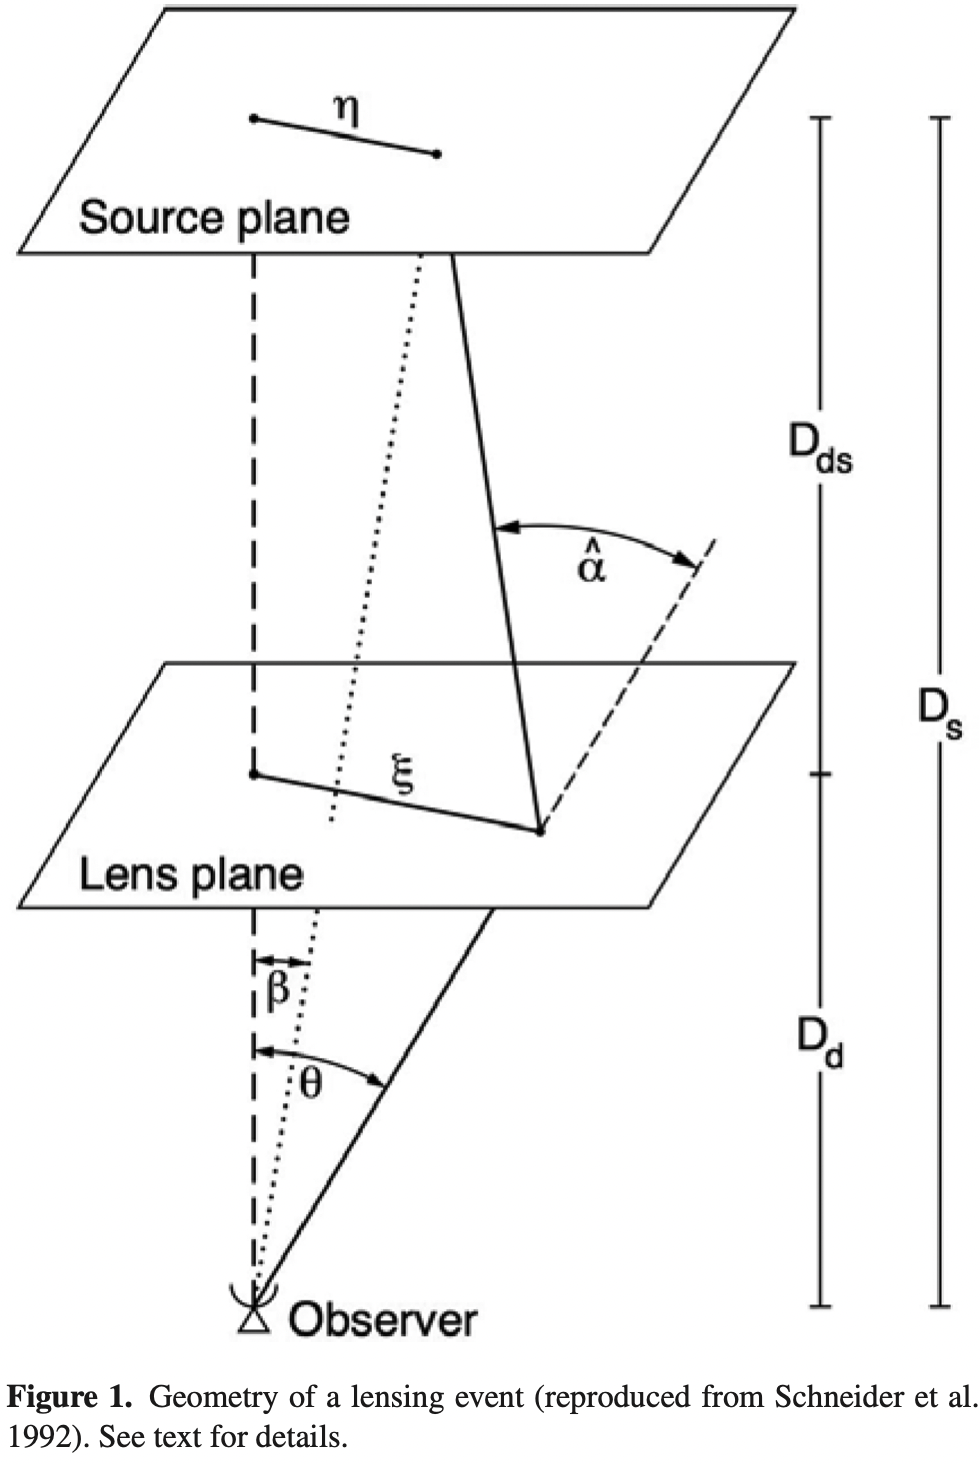
\includegraphics[width=1.5in]{Figures/lens.png}

  }


  \frame{
\vspace{-0.25in}
    \frametitle{Huygen's Principle: Path Integral}
    \begin{itemize}
        \item $A=\int e^{i S(\theta,\mu)} d\theta$ 
        \item $S=\nu [(\theta-\mu)^2+\Psi(\theta)]$
        \item Highly oscillatory integral, even for $\Psi=0$
        \item Stationary phase points: $\partial_\theta S=0$ leads to (complex)
          Eikonal images $\theta_i$.
        \item flux/phase through curvature expansion (known as {\it
            steepest descent}): exact as $\nu \rightarrow \infty$
        \item Geometric limit considers only {\it Real} $\theta_i$ and
          absolute value of the action $S$, giving up phase
          information
        \item Geometric optics applicable at short wavelengths for
          extended sources
          (e.g. optical gravitational lensing of finite size sources,
          stars)     
          \item roughly 1/4 of the degrees of freedom of Eikonal 
    \end{itemize}
  }


  \frame{
\vspace{-0.5in}
    \frametitle{Oscillations!}
    \begin{itemize}
    \item in 2-D axisymmetry, in empty space, action integral 
    \item $\int \exp(i r^2) r \d r = \int \sin(r^2) r \d r$
    \item numerical interpretation unclear, gets worse in higher dimensions
    \end{itemize}
  }

  \frame{
\vspace{-0.5in}
    \frametitle{Imaginary Images}
    \begin{itemize}
    \item consider ``rational lens'' potential $\psi(\theta)=\alpha/(1+\theta^2)$
    \item Geometric/eikonal images at $\psi'=\theta$
    \item 5 roots.  1 or 3 real roots, rest imaginary
    \item P-L: at most one imaginary image contributes!
    \item imaginary image can be brighter than unlensed real image
    \end{itemize}
  }


  \frame{
%\vspace{-0.5in}
    \frametitle{Rational 1-D lens}
\begin{center}
\includegraphics[width=3.1in]{Figures/theta-beta.eps}
\end{center}
  }

  \frame{
\vspace{-0.5in}
    \frametitle{Picard-Lefschetz Theory}
    \begin{itemize}
    \item descend integral along real line along Morse function Im(S)
    \item contour deforms into finite number of Thimbles of constant
      phase with maximum at saddle point (extrema $dS=0$)
    \item correctly identifies relevant saddle points
    \item resolves numerical challenges of oscillatory integral
    \item complex analysis works in multiple variables
    \item elevates concept of ``image'' deep into wave optics
    \item multiple public implementations (Feldbrugge+, Jow+)
    \end{itemize}
  }



  \frame{
\vspace{-0.5in}
    \frametitle{Picard-Lefschetz Theory}

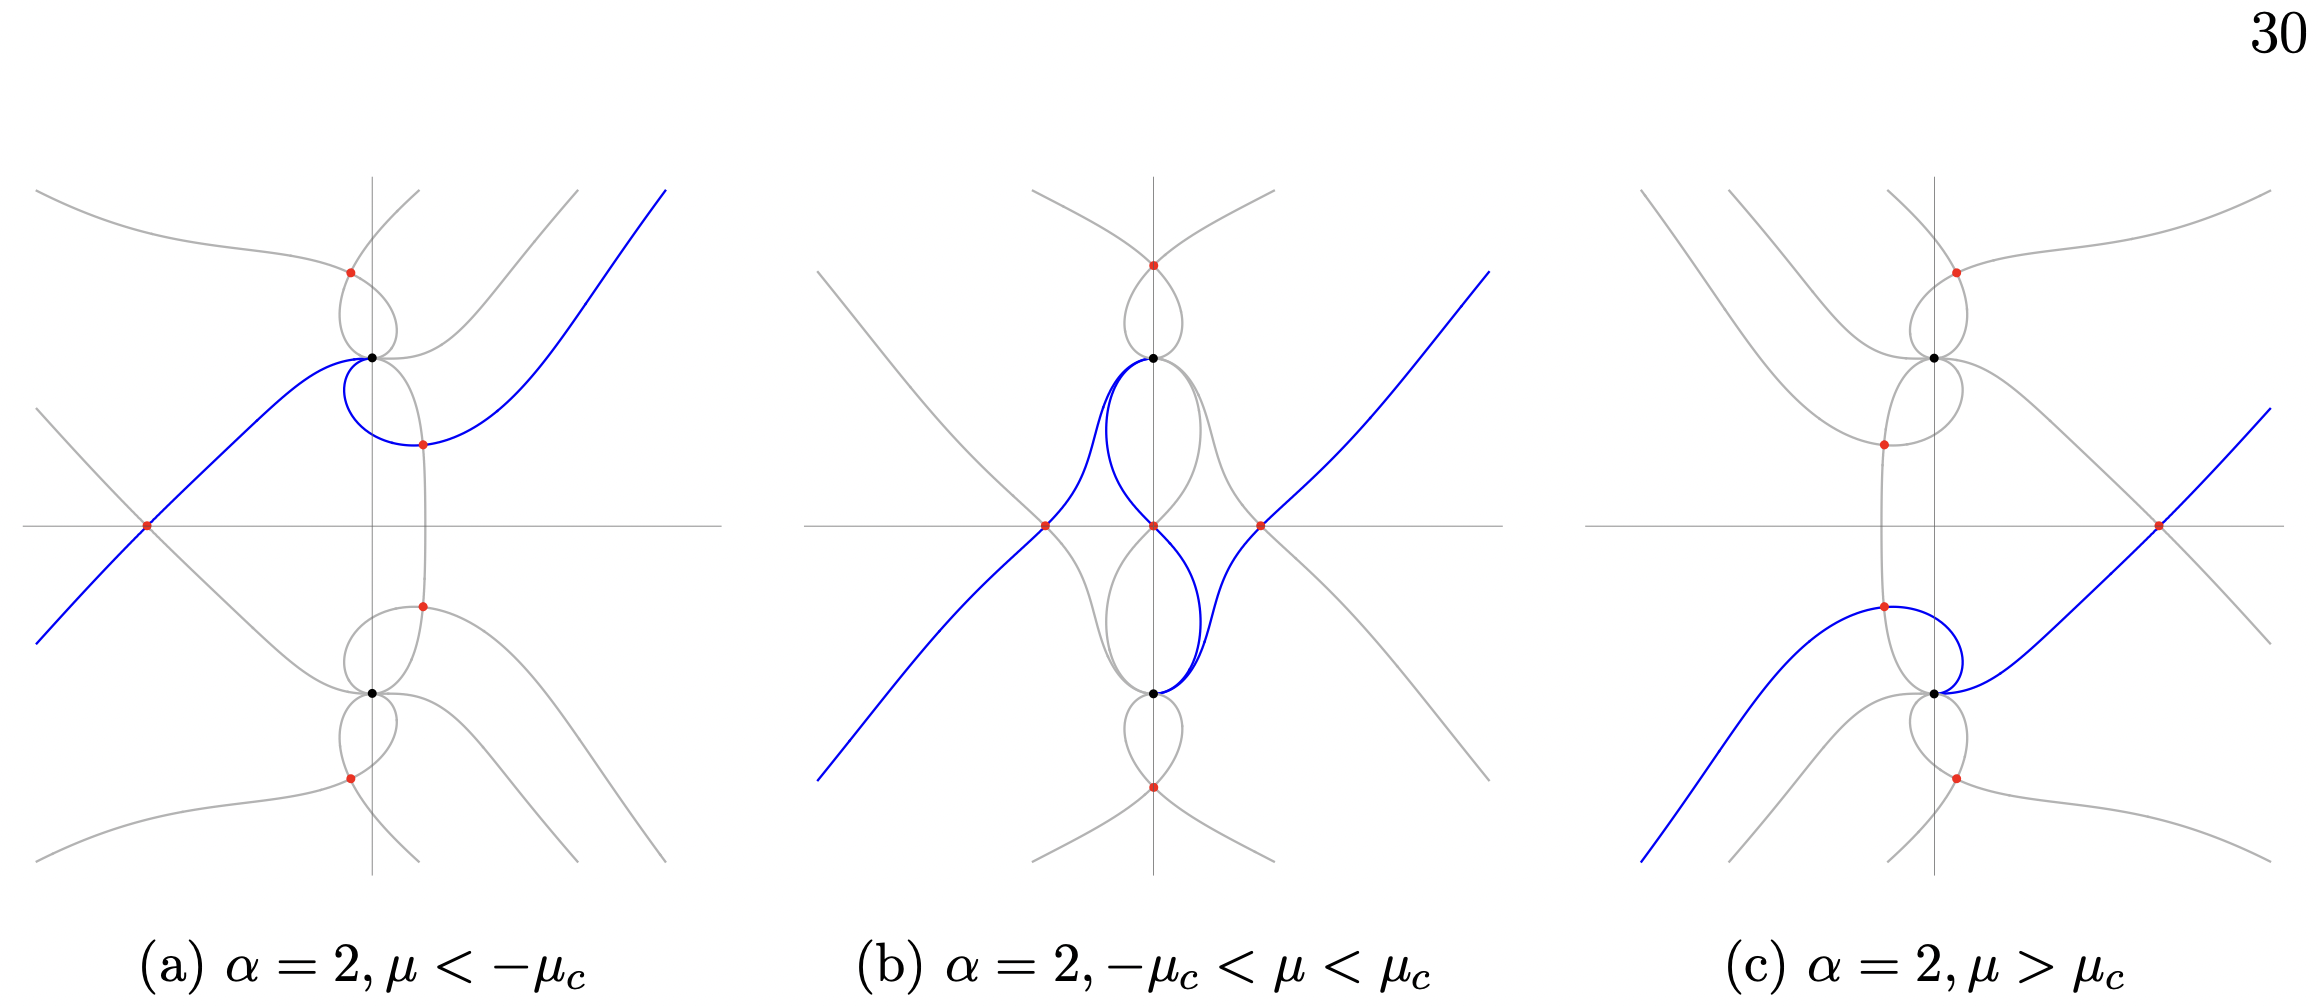
\includegraphics[width=4.5in]{Figures/thimbles.png}

Feldbrugge+2019
  }


  \frame{
\vspace{-0.5in}
    \frametitle{Imaginary classical paths}
    \begin{itemize}
    \item PL interpretation: oscillatory integral is sum over thimbles
    \item each thimble has exactly one stationary point (maxima, classical path)
    \item path integral is sum over thimbles
    \item eikonal limit is quadratic expansion at maxima
    \item alternative interpretation of quantum mechanics from
      classical mechanics:
    \item sum over real and imaginary classical paths
    \item Turok 2014, Cherman+ 2014, Mou+ 2014
    \end{itemize}
  }

  \frame{
\vspace{-0.5in}
    \frametitle{New Observables}
    \begin{itemize}
    \item weak lensing: imaginary image allows time delay measurement (Jow+21)
    \item strong lensing: delay measurements enable measurement of
      co-linearity (Jow++21)
    \item microlensing: instant time delay, planets (Jow+20)
    \item macrolensing: potentially nano-second delay -- universe
      expands! (Wucknitz+21)
    \item dimensionless strain picoseconds/years $h\sim \Delta t/t \sim 10^{-20}$:
      competitive with LIGO, etc
    \end{itemize}
  }


  \frame{
%\vspace{-0.5in}
    \frametitle{A2 fold}
\begin{center}
\vspace{-0.3in}
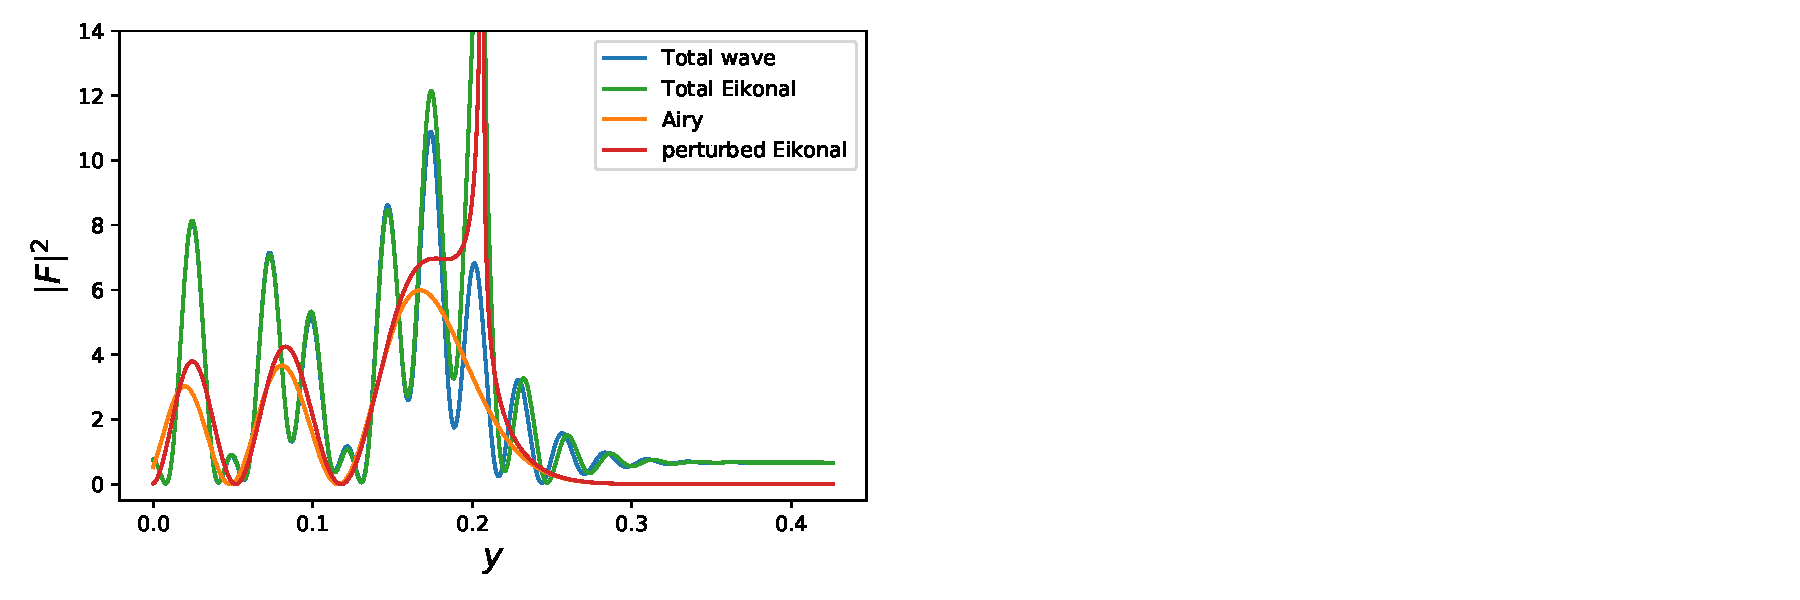
\includegraphics[width=4.5in]{Figures/rational_fold_crossing.pdf}
\end{center}
  }


  \frame{
\vspace{-0.5in}
    \frametitle{Stokes Phenomenon}
    \begin{itemize}
    \item Imaginary images (dis-)appear at caustics and Stokes lines
    \item in single image regime, imaginary image disappears on-axis
    \end{itemize}
  }


  \frame{
%\vspace{-0.5in}
    \frametitle{weak lens}
\begin{center}
\vspace{-0.3in}
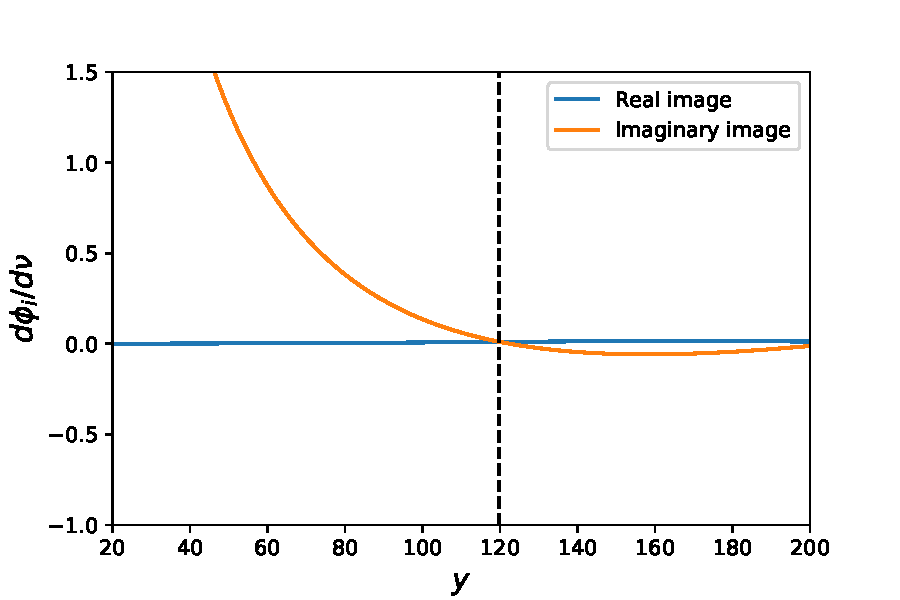
\includegraphics[width=4.5in]{Figures/stokes_phase_gradient.pdf}
\end{center}
  }

  \frame{
\vspace{-0.5in}
    \frametitle{Macrolensing}
    \begin{itemize}
    \item Wucknitz+ 2021
    \item alternate approach to cosmography
    \item triangulation: lens model+time delay measurement = $H_0$
    \item weak link has been lens model
    \item Wave optics: time delay observable to nanoseconds
    \item For repeating FRB, dominated by galaxy transverse
      motion. then cosmic expansion
    \item individual macrolens images split into microlens images by stars
    \end{itemize}
  }



  \frame{
\vspace{-0.5in}
    \frametitle{Discussion}
    \begin{itemize}
    \item Eikonal effects applicable to compact radio sources,
      e.g. FRBs, pulsars
    \item full wave
effect dominates for long wavelengths as Fresnel scale is bigger then Einstein radius
    \item down to planet size
    \item gravitational waves:  LIGO, LISA, PTA
    \end{itemize}
  }



  \frame{
\vspace{-0.5in}
    \frametitle{Current status}
    \begin{itemize}
    \item Eikonal: pulsar scintillation, wind magnification (Main+ 2018)
    \item full wave optics: pulsar wind lensing, solar wind (IPS)
    \end{itemize}
  }

\frame{
    \frametitle{Microscope}
     \vspace{-0.65in}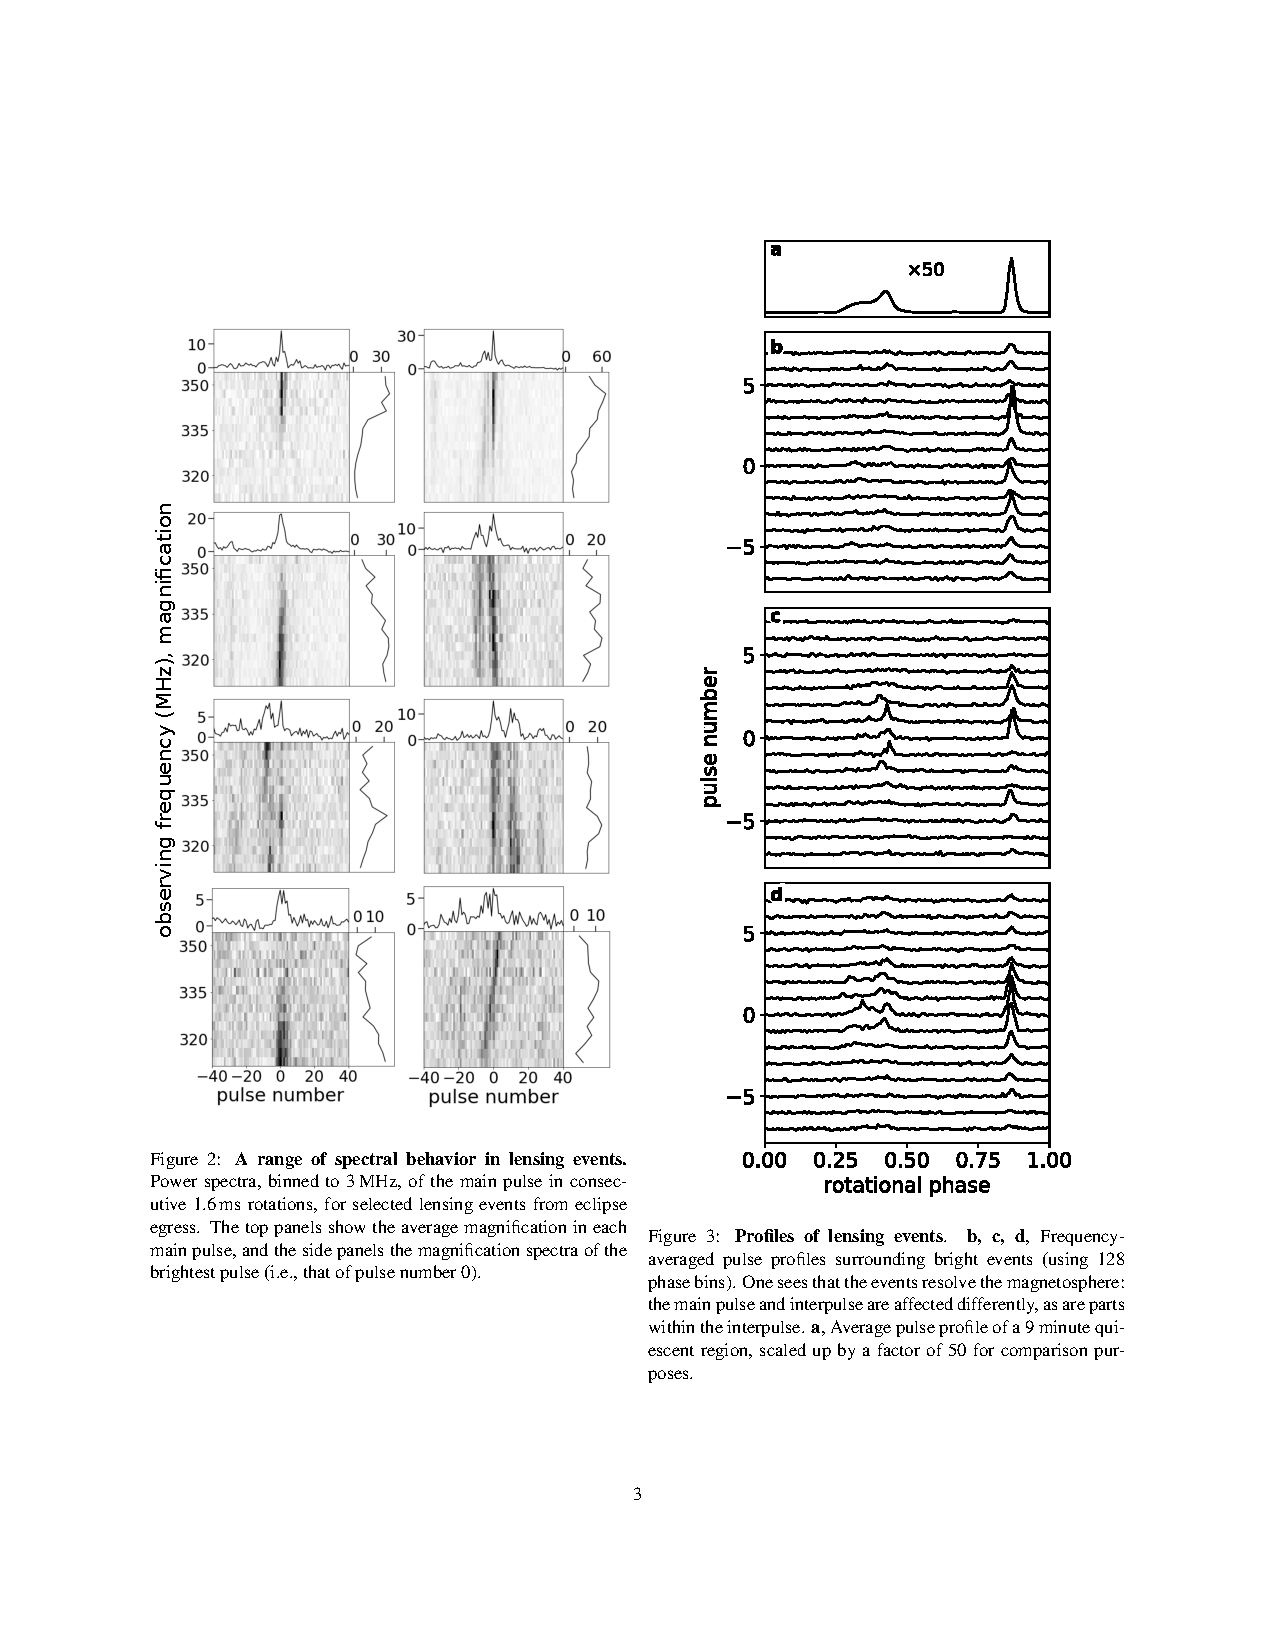
\includegraphics[width=0.75\textwidth]{Figures/bwlens.pdf}
}



  \frame{
\vspace{-0.5in}
    \frametitle{Conclusions}
    \begin{itemize}
    \item wave optics changes nature of observables: one of the potentially most
      precise measurements in physics
    \item coherent radio waves (FRBs, pulsars): described by Eikonal
      away from caustics/catastrophies
    \item long wavelength GW (LIGO, LISA, PTA): full wave effects, P-L theory
    \item importance of imaginary images
    \end{itemize}
  }

\end{document}
